\chapter{Continuous Random Variables}

The probability models we used earlier were discrete. Starting from this chapter, we will discuss some non-discrete probability models.

Suppose a postal package is to be delivered to you between noon and 1:00 pm. You have to leave home between 12:30 to 12:45 pm.

What is the probability you miss the delivery?

\section{Uniform Random Variable}
This question is quite simple, and we can immediately see that the answer is \(\frac{15}{60}\). However, how can we define a probability model here?

\begin{definition}[Uniform Random Variable]
    A uniform random variable \(T\) over interval \([0, 1]\) satisfies 
    \[
        \mathbb{P}(T \leq t) = \begin{dcases}
            0, &\text{ if } t \leq 0 ,\\
            t, &\text{ if } 0 < t \leq 1 ,\\
            1, &\text{ if } 1 < t.
        \end{dcases}
    \]
\end{definition}

Based on the above definition, we can calculate the following: 

\(
\begin{aligned}
    \mathbb{P}(T > \dfrac{1}{2}) &= 1 - \mathbb{P}(T \leq \dfrac{1}{2}) = 1 - \dfrac{1}{2} = \dfrac{1}{2} \\
    \mathbb{P}(T > \dfrac{3}{4}) &= 1 - \mathbb{P}(T \leq \dfrac{3}{4}) = 1 - \dfrac{3}{4} = \dfrac{1}{4} \\
    \mathbb{P}(\dfrac{1}{2} < T \leq \dfrac{3}{4}) &= \mathbb{P}(T > \dfrac{1}{2}) - \mathbb{P}(T > \dfrac{3}{4}) = \dfrac{1}{2} - \dfrac{1}{4} = \dfrac{1}{4}
\end{aligned}
\) 

\begin{eg}[Continuous Random Variables and Zero Probability for Points]~ 
    Consider a Uniform(\([0, 1]\)) random variable \(T\). 

    1. \(\mathbb{P}(T \leq 0.3) = 0.3\) 

    2. \(\mathbb{P}(T = 0.3) = 0\)
        
    Assume that \(\mathbb{P}(T = 0.3) = \varepsilon > 0\), \(\mathbb{P}(T \leq 0.3 - \frac{\varepsilon}{4}) = 0.3 - \frac{\varepsilon}{4}\), \(\mathbb{P}(T \leq 0.3 + \frac{\varepsilon}{4}) = 0.3 + \frac{\varepsilon}{4}\)

    Above gives \(\mathbb{P}(0.3 - \frac{\varepsilon}{4} < T < 0.3 + \frac{\varepsilon}{4}) = \mathbb{P}(T \leq 0.3 + \frac{\varepsilon}{4}) - \mathbb{P}(T \leq 0.3 - \frac{\varepsilon}{4}) = \frac{\varepsilon}{2}\) 

    However, for \(\mathbb{P}(T = 0.3) \subseteq \mathbb{P}(0.3 - \frac{\varepsilon}{4} < T < 0.3 + \frac{\varepsilon}{4})\), we have \(\varepsilon < \frac{\varepsilon}{2}\), which by contradiction shows that \(\mathbb{P}(T = 0.3) = 0\)

    3. \(\mathbb{P}(T < 0.3) = \mathbb{P}(T \leq 0.3) - \mathbb{P}(T = 0.3) = 0.3\)
\end{eg}

Above shows that the probability mass function (PMF) does not make much sense because \(\mathbb{P}(T = t) = 0\) for every \(t\).

\section{Cumulative Distribution Function (CDF)}
The Cumulative Distribution Function works for both discrete and continuous probabilities.
\begin{definition}[Cumulative Distribution Function (CDF)]
  The cumulative distribution function (CDF) \(F\) of a random variable \(X\) is:
  \[
    F(x) = \mathbb{P}(X \leq x)
  \]
\end{definition}

Every CDF \(F:\mathbb{R} \to [0, 1]\) must satisfy the following properties:

1. \(F\) is monotonically increasing: \(x \leq y \Longrightarrow F(x) \leq F(y)\)

2. \(\lim_{n \to -\infty} F(x) = 0\) 

3. \(\lim_{n \to +\infty} F(x) = 1\) 

\begin{eg}
    Find the CDF of a Geometric(\(p = \frac{1}{2}\)) random variable.

    \textbf{Solution:} 
    \[
        F(k) = \mathbb{P}[X \leq k] = 1 - \mathbb{P}[X > k] = 1 - (1 - p)^k
    \]
\end{eg}

By observation, we see that the CDF of a Uniform random variable over interval \([0, 1]\) is 
\[
    F(x) = \mathbb{P}(X \leq x) = \begin{dcases}
        0, &\text{ if } x \leq 0 ,\\
        x, &\text{ if } 0 < x \leq 1 ,\\
        1, &\text{ if } 1 < x.
    \end{dcases}
\]

\subsection{Probability Density Function (PDF)}
\begin{definition}[Probability Density Function (PDF)]
    For a continuous random variable \(X\), we define its probability density function (PDF) \(f\) as the derivative of its CDF:
    \[
        f(X) \coloneqq \lim_{\delta \to 0} \dfrac{\mathbb{P}(x \leq X \leq x + \delta)}{\delta}= \lim_{\delta \to 0} \dfrac{F(x + \delta) - F(x)}{\delta} = \frac{\mathrm{d}F(x)}{\mathrm{d}x}  
    \]

    \begin{remark}
        PDF is not probability, it is the rate of probability. 
    \end{remark}
\end{definition}

For a small \(\delta > 0\), we know \(F(x + \delta) - F(x) \approx f(x)\delta\) and so for small \(\delta \), 
\[
    \mathbb{P}(x \leq X \leq x + \delta) \approx f(x)\delta
\]
For example, 
\[
    F(x) = \begin{dcases}
        0, &\text{ if } x < 0 ,\\
        x, &\text{ if } 0 \leq  x \leq 1 ,\\
        1, &\text{ if } 1 < x.
    \end{dcases}
    \quad\Longrightarrow\quad 
    f(x) = \begin{dcases}
        0, &\text{ if } x < 0 ,\\
        1, &\text{ if } 0 \leq x \leq 1 ,\\
        0, &\text{ if } 1 < x.
    \end{dcases}
\]

\begin{eg}
    The CDF of random variable \(X\) is \(F(x) = \begin{dcases}
        1 - \frac{1}{x^2}, &\text{ if } x > 1 \\
        0, &\text{ if } x \leq 1 
    \end{dcases}\). 
    
    Find the PDF of \(X\).

    \textbf{Solution:} 
    First, we need to verify whether it is a valid CDF. Since it satisfies the three properties, we can then determine the PDF of \(X\).
    \[
        f(x) = \frac{\mathrm{d}F(x)}{\mathrm{d}x} = \begin{dcases}
            \dfrac{2}{x^3}, &\text{ if } x > 1 \\
            0 , &\text{ if } x \leq 1 
        \end{dcases}
    \] 
\end{eg}
\begin{remark}
    A PDF can take any non-negative value \(f(x) \geq 0\) and its value can be greater than 1.
\end{remark}

\begin{minipage}{0.5\textwidth}
    \centering
    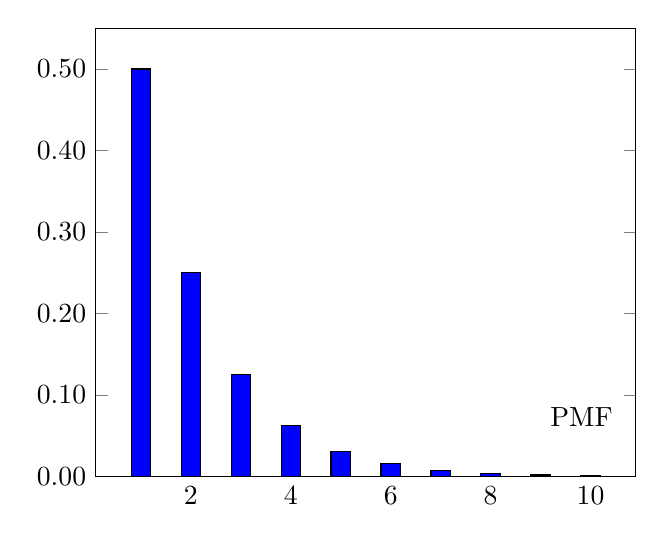
\begin{tikzpicture}
        \begin{axis}[
            ymin=0,
            ymax=0.55,
            xtick={0,2,...,10},
            ytick={0,0.1,...,0.5},
            samples at={1,...,10},
            xtick style={draw=none},
              yticklabel style={
                  /pgf/number format/fixed,
                  /pgf/number format/fixed zerofill,
                  /pgf/number format/precision=2,
            },   
            domain=1:10,
            samples=10,
        ]
        % Define p, probability of success
        \pgfmathsetmacro{\p}{0.5}
        
        % Plot the PMF of the geometric distribution
        \addplot [
          ybar=0pt,
          bar width=7pt,
          fill=blue,
          mark=none,
      ] {(\p*(1-\p)^(x-1))};
      % Add "discrete CDF" label
      \node[anchor=south west] at (axis cs:9,0.05) {PMF};
        \end{axis}
    \end{tikzpicture}
\end{minipage}
\begin{minipage}{0.5\textwidth}
    \centering
    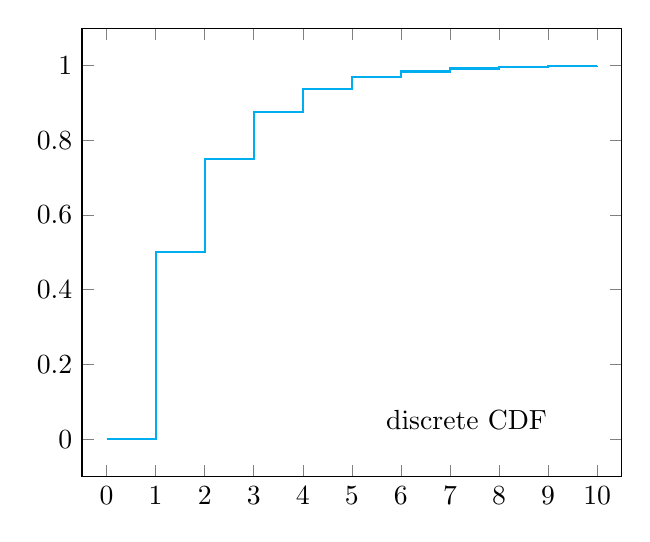
\begin{tikzpicture}
    \begin{axis}[
        axis lines=box,
        xtick={0,1,...,10},
        ytick={0,0.2,...,1},
        ymin=-0.1, ymax=1.1,
        xmin=-0.5, xmax=10.5,
        every axis x label/.style={at={(ticklabel* cs:1)}, anchor=north},
        every axis y label/.style={at={(ticklabel* cs:1)}, anchor=east},
    ]
        % Plot the stepwise CDF
        \addplot[
            thick,
            cyan,
            const plot
        ] coordinates {
            (0, 0)
            (1, 0.5)
            (2, 0.75)
            (3, 0.875)
            (4, 0.9375)
            (5, 0.96875)
            (6, 0.984375)
            (7, 0.9921875)
            (8, 0.99609375)
            (9, 0.998046875)
            (10, 0.999023437)
        };

        % Add "discrete CDF" label
        \node[anchor=south west] at (axis cs:5.5,0) {discrete CDF};
    \end{axis}
\end{tikzpicture}
\end{minipage}

\begin{minipage}{0.5\textwidth}
    \centering
    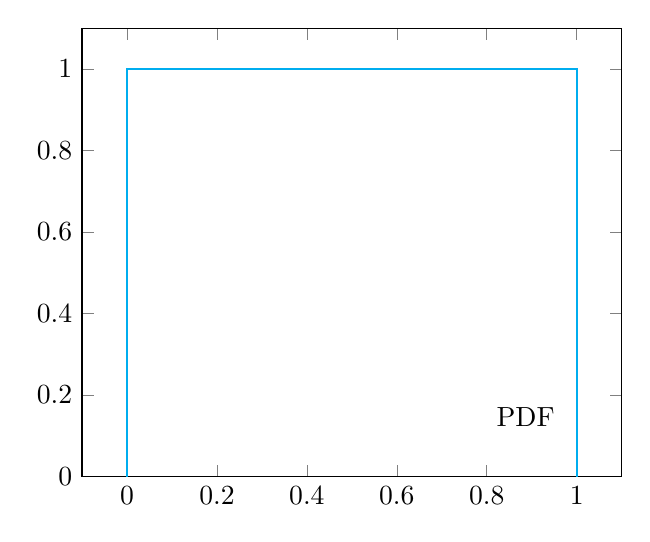
\begin{tikzpicture}
        \begin{axis}[
            axis lines=box,
            xtick={0,0.1,...,1.0},
            ytick={0,0.2,...,1.0},
            xmin=-0.1, xmax=1.1,
            ymin=0.0, ymax=1.1,
            xtick={0,0.2,...,1.0},
            ytick={0,0.2,...,1.0},
            samples at={0.0,...,1.0},
        ]
            % Plot the stepwise CDF
            \addplot[
                thick,
                cyan,
                const plot
            ] coordinates {
                (0.0, 0.0)
                (0.0, 1.0)
                (0.1, 1.0)
                (0.2, 1.0)
                (0.3, 1.0)
                (0.4, 1.0)
                (0.5, 1.0)
                (0.6, 1.0)
                (0.7, 1.0)
                (0.8, 1.0)
                (0.9, 1.0)
                (1.0, 0.0)
            };
            % Add "discrete CDF" label
            \node[anchor=south west] at (axis cs:0.8,0.1) {PDF};
        \end{axis}
    \end{tikzpicture}
\end{minipage}
\begin{minipage}{0.5\textwidth}
    \centering
    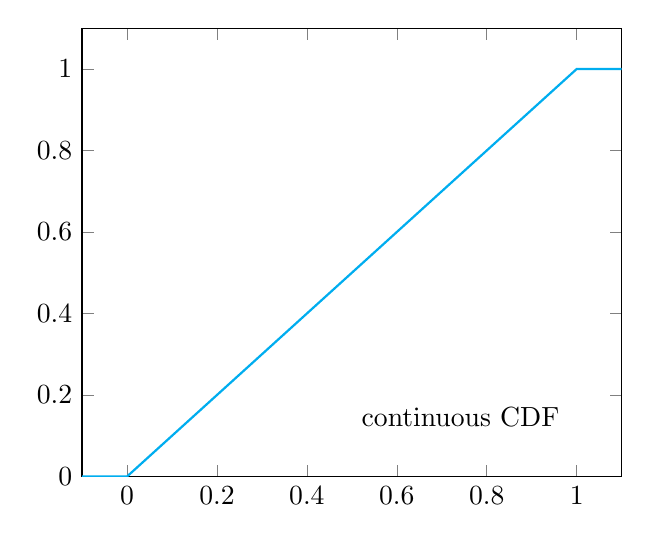
\begin{tikzpicture}
        \begin{axis}[
            axis lines=box,
            xtick={0,0.1,...,1.0},
            ytick={0,0.2,...,1.0},
            xmin=-0.1, xmax=1.1,
            ymin=0.0, ymax=1.1,
            xtick={0,0.2,...,1.0},
            ytick={0,0.2,...,1.0},
            samples at={0.0,...,1.0},
        ]
            % Plot the stepwise CDF
            \addplot[
                thick,
                cyan,
            ] coordinates {
                (-0.1, 0.0)
                (0.0, 0.0)
                (1.0, 1.0)
                (1.1, 1.0)
            };
            % Add "discrete CDF" label
            \node[anchor=south west] at (axis cs:0.5,0.1) {continuous CDF};
        \end{axis}
    \end{tikzpicture}
\end{minipage}

\subsection{Integral of PDF and Probability Calculation}
For a continuous random variable \(X\) , the probability of an event \(E\) can be calculated using the integral of PDF \(f\). Therefore,
\begin{itemize}
    \item \(\mathbb{P}(E) = \int_E f(x)dx\) 
    \item \(\mathbb{P}(X \leq t) = \int_{-\infty}^t f(x)dx\) 
    \item \(\int_{-\infty}^{\infty} f(x)dx = 1\) 
\end{itemize}

To summarize, we have 
\begin{table}[H]
    \centering
    \begin{tabular}{c c c}
        \toprule
             & PMF \(f(x)\)  & PDF \(f(x)\)  \\
        \midrule
            \(\mathbb{P}(X \leq a)\)  & \(\sum_{x \leq a} f(x)\)  & \(\int_{-\infty}^a f(x)dx \)   \\[5pt]
            \(\mathbb{E}[X]\) & \(\sum_{x} xf(x)\) & \(\int_{-\infty}^{\infty} xf(x)dx \)  \\[5pt]
            \(\mathbb{E}[X^2]\) & \(\sum_{x} x^2f(x)\) & \(\int_{-\infty}^{\infty} x^2f(x)dx \)  \\[5pt]
            \(\Var[X]\) & \(\mathbb{E}[X^2] - \mathbb{E}[X]^2\)  & \(\mathbb{E}[X^2] - \mathbb{E}[X]^2\)  \\[5pt]
            \(\Var[X]\) & \(\sum_{x} (x - \mu)^2 f(x)\)  & \(\int_{-\infty}^{\infty} (x - \mu)^2 f(x)dx \)  \\[5pt]
        \bottomrule
    \end{tabular}
\end{table} 

\begin{eg}
    Find the expected value and variance of a Uniform(\([0, 1]\)) random variable.

    \textbf{Solution:} 
    \[
        f(x) = \begin{dcases}
            0, &\text{ if } x < 0 ,\\
            1, &\text{ if } 0 \leq x \leq 1 ,\\
            0, &\text{ if } 1 < x.
        \end{dcases}
    \]
    \[
    \begin{aligned}
        \mathbb{E}(x) &= \int_{-\infty} ^{\infty} xf(x)dx = \int_{0}^{1} x \cdot 1 dx = \dfrac{x^2}{2} \Big|_0^1 = \frac{1}{2} \\
        \mathbb{E}(x^2) &= \int_{-\infty} ^{\infty} x^2f(x)dx = \int_{0}^{1} x^2 \cdot 1 dx = \dfrac{x^3}{3} \Big|_0^1 = \frac{1}{3} \\
        \Var(x) &= \mathbb{E}[X^2] - \mathbb{E}[X]^2 = \dfrac{1}{3} - (\dfrac{1}{2})^2 = \dfrac{1}{12}
    \end{aligned}
    \]
\end{eg}

Consider a Uniform random variable X over interval \([a, b]\), i.e., 
\[
    F(x) = \begin{dcases}
        0, &\text{ if } x < a \\
        \frac{x - a}{b - a}, &\text{ if } a \leq x \leq b \\
        1 , &\text{ if } b < x
    \end{dcases}
\]
Then,

1. The PDF of \(X\) is \(f(x) = \begin{dcases}
        0, &\text{ if } x < a \\
        \frac{1}{b - a}, &\text{ if } a \leq x \leq b \\
        0 , &\text{ if } b < x
    \end{dcases}\) 
    \[
        \text{If}\ f(x) = c\ \text{for}\ a \leq x \leq b,\ \text{since}\ \int_{-\infty} ^{\infty} f(x)dx = 1 \Rightarrow c(b - a) = 1 \Rightarrow c = \frac{1}{b - a}
    \]
2. The expected value of \(X\) is \(\mathbb{E}[X] = \dfrac{a + b}{2}\)
    \[
        \mathbb{E}[X] = \int_{-\infty} ^{\infty} xf(x)dx = \int_{a} ^{b} \dfrac{x}{b - a}dx = \dfrac{1}{b - a}\int_{a} ^{b} xdx = \dfrac{x^2}{2(b - a)} \Big|_a^b = \dfrac{a + b}{2}
    \]
3. The variance of \(X\) is \(\Var[X] = \dfrac{(b - a)^2}{12}\)
    
    Let \(Y\) be Uniform(\([0, 1]\)) \(\rightarrow \mathbb{E}[Y] = \frac{1}{2}, \Var(Y) = \frac{1}{12}\) 

    Let \(Z = (b - a)Y + a\), which gives Uniform(\([a, b]\)) 
    \[
    \begin{aligned}
        \mathbb{E}[Z] &= (b - a)\mathbb{E}[Y] + a = \dfrac{b + a}{2} \\
        \Var[Z] &= (b - a)^2 \Var[Y] = \dfrac{(b - a)^2}{12}
    \end{aligned}
    \]

\section{Exponential Random Variable}

Consider rain is falling on your head at a rate of \(\lambda\) drops/sec. How long do we wait until the next drop?

We can first divide 1 second to n sub-intervals, then the probability of rain drop would be \(\frac{\lambda}{n}\). 

Then we have 
\[
    \dfrac{\mathbb{P}(T = \frac{t}{n})}{\frac{1}{n}} = \frac{\frac{\lambda}{n}\left(1 - \frac{\lambda}{n}\right)^{t-1}}{\frac{1}{n}} \quad(\text{Let}\ t = ns) = \lambda\left(1 - \dfrac{\lambda}{n}\right)^{ns-1}
\]
\[
    \lim_{n \to \infty} \dfrac{\mathbb{P}(T = \frac{t}{n})}{\frac{1}{n}} = \lim_{n \to \infty} \lambda\left(1 - \dfrac{\lambda}{n}\right)^{ns-1} = \lim_{n \to \infty} \lambda\left(1 - \dfrac{\lambda}{n}\right)^{ns}\left(1 - \dfrac{\lambda}{n}\right)^{-1} = \lambda \left(\lim_{n \to \infty} \left(1 - \dfrac{\lambda}{n}\right)^n\right)^s = \lambda e^{-\lambda s}
\]

\begin{definition}[Exponential Random Variable]
    An Exponential(\(\lambda\)) random variable has the following PDF: 
    \[
        f(x) = \begin{dcases}
            \lambda e^{-\lambda x} , &\text{ if }  x \geq 0\\
            0 , &\text{ if } x < 0
        \end{dcases}
    \]
\end{definition}

To check the validity of the above, we proceed as follows:
\[
    \int_{-\infty}^{\infty} f(x)dx = \int_0^{\infty} \lambda e^{-\lambda x} dx = -e^{-\lambda x} \Big|_0^{\infty} = 1
\]

The Exponential(\(\lambda\)) random variable \(X\) satisfies:

1. The CDF of \(X\) is \(F(x) = 1 - e^{-\lambda x}\) (\(x \geq 0\))
\[
    F(x) = \int_{-\infty}^x f(x) dx = \int_{0}^x \lambda e^{-\lambda x} dx = -e^{-\lambda x} \Big|_0^x = 1 - e^{- \lambda x}
\]
2. The expected value of \(X\) is \(\mathbb{E}[X] = \frac{1}{\lambda}\)
\[
\mathbb{E}[X] = \int_{-\infty }^{\infty} xf(x) dx = \int_{0}^{\infty} \lambda x e^{-\lambda x} dx = \left[-xe^{-\lambda x} - \dfrac{1}{\lambda }e^{-\lambda x}\right]_0^{\infty} = 0 - (0 -\dfrac{1}{\lambda }) = \dfrac{1}{\lambda}
\]
3. The variance of \(X\) is \(\Var[X] = \dfrac{1}{\lambda^2}\) 

Exponential and Geometric Random Variables can be related as the following:
\[
    \lim_{n \to \infty} \dfrac{1}{n} \text{Geometric}(\dfrac{\lambda}{n}) = \text{Exponential}(\lambda) 
\]

The exponential distribution has the memoryless property, which says that future probabilities do not depend on any past information

\begin{eg}[Memoryless Property of Exponential Distribution]~ 

    Buses arrive at a rate of one in 5 minutes. 

    (a) A bus arrives now. How likely are you to wait at least 5 minutes for the next bus?

    \textbf{Solution:} 
    Let \(X = \) time to wait until the next bus arrives. Given that \(\mathbb{E}[X] = 5, \frac{1}{\lambda} = 5, \lambda = 0.2\) 
    \[
        \mathbb{P}(X \geq 5) = 1 - F_X(5) = 1 - (1 - e^{-\lambda x}) = e^{-0.2 \times 5} = e^{-1}
    \]

    (b) The last bus arrived 5 minutes ago. How likely are you to wait at least 5 minutes from now for the next bus to come?

    \textbf{Solution:} 
    \[
        \mathbb{P}(X \geq 10 \vert X \geq 5) = \dfrac{\mathbb{P}(X \geq 10 \cap X \geq 5)}{\mathbb{P}(X \geq 5)} = \dfrac{\mathbb{P}(X \geq 10)}{\mathbb{P}(X \geq 5)} = \dfrac{e^{-0.2 \times 10}}{e^{-0.2 \times 5}} = e^{-1}
    \]
\end{eg}

The Exponential distribution is memoryless (the past has no effects on
its future), which means for every exponential random variable \(X\) and
constants \(s, t \geq 0\): 
\[
    \mathbb{P}(X \geq s + t \vert X \geq t) = \mathbb{P}(X \geq s)
\] 
\begin{proof}
    \[
        \mathbb{P}(X \geq s + t \vert X \geq t) = \dfrac{\mathbb{P}(X \geq s + t \cap X \geq t)}{\mathbb{P}(X \geq t)} = \dfrac{\mathbb{P}(X \geq s + t)}{\mathbb{P}(X \geq t)} = \dfrac{e^{-(s + t)\lambda}}{e^{-t\lambda}} = e^{-s\lambda} = \mathbb{P}(X \geq s)
    \]
\end{proof}

\newpage
\section{Normal Distribution (Gaussian Random Variable)}
\subsection{Normal Random Variable}
We see from the following that as \(n\) increases, the shape converges to a bell shape curve.

\begin{minipage}{0.5\textwidth}
    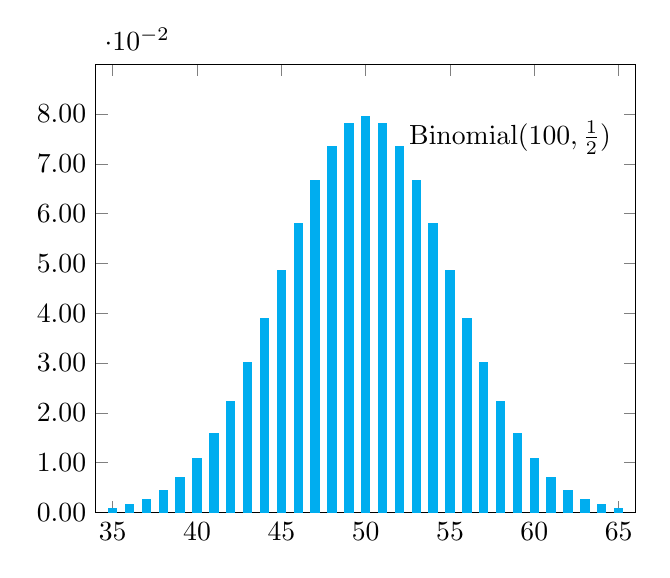
\begin{tikzpicture}
    \begin{axis}
    [
        % Define probability distribution functions
        declare function={
            binom(\n,\p) = \n!/(x!*(\n-x)!)*\p^x*(1-\p)^(\n-x);
            normal(\m,\s) = 1/(\s*sqrt(2*pi))*exp(-((x-\m)^2)/(2*\s^2));
        },
        % Plotting options
        xmin=34, xmax=66,
        ymin=0.0, ymax=0.09,
        samples at={35,...,65},
        xtick={35,40,...,65},
        ytick={0,0.01,...,0.08},
        yticklabel style={
            /pgf/number format/fixed,
            /pgf/number format/fixed zerofill,
            /pgf/number format/precision=2,
        },   
    ]
    
    % Plot Binomial Distribution
    \addplot [draw=cyan,ybar=0pt,bar width=3pt,fill=cyan] {binom(100,0.5)};
    % Add "discrete CDF" label
    \node[anchor=south west] at (axis cs:52,0.07) {Binomial(\(100, \frac{1}{2}\))};
    \end{axis}
\end{tikzpicture}
\end{minipage}
\begin{minipage}{0.5\textwidth}
    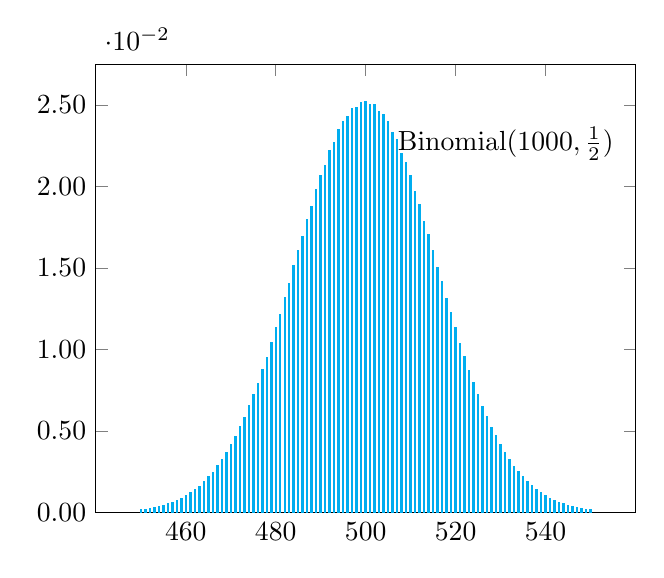
\begin{tikzpicture}
    \begin{axis}
    [
        % Define probability distribution functions
        declare function={
            binom(\n,\p) = \n!/(x!*(\n-x)!)*\p^x*(1-\p)^(\n-x);
            normal(\m,\s) = 1/(\s*sqrt(2*pi))*exp(-((x-\m)^2)/(2*\s^2));
        },
        % Plotting options
        xmin=440, xmax=560,
        ymin=0.0, ymax=0.0275,
        samples at={450,...,550},
        xtick={460,480,...,540},
        ytick={0,0.005,...,0.025},
        yticklabel style={
            /pgf/number format/fixed,
            /pgf/number format/fixed zerofill,
            /pgf/number format/precision=2,
        },   
    ]
    
    % Plot Binomial Distribution
    \addplot [draw=cyan,ybar=0pt,bar width=0.5pt,fill=cyan] {binom(1000,0.5)};
    % Add "discrete CDF" label
    \node[anchor=south west] at (axis cs:505,0.021) {Binomial(\(1000, \frac{1}{2}\))};
    \end{axis}
\end{tikzpicture}
\end{minipage}

\begin{definition}[Normal Distribution]
    We define normal (Gaussian) probability density function (PDF) with the parameters \(\mu\) and \(\sigma^2\) as 
    \[
        f(x) \coloneqq \dfrac{1}{\sqrt{2\pi \sigma ^2}}e^{-\frac{(x - \mu)^2}{2\sigma^2}}
    \]
\end{definition}
\begin{remark}
    From calculus we know that 
    \[
        \int_{x = -\infty}^{\infty} \dfrac{1}{\sqrt{2\pi \sigma ^2}}e^{-\frac{(x - \mu)^2}{2\sigma^2}} dx = \dfrac{1}{\sqrt{2\pi \sigma ^2}}\int_{x = -\infty}^{\infty} e^{-\frac{(x - \mu)^2}{2\sigma^2}} dx = 1 \Longrightarrow \int_{x = -\infty}^{\infty} e^{-\frac{(x - \mu)^2}{2\sigma^2}} dx = \sqrt{2\pi \sigma ^2}
    \]
    which makes it easier for the calculation of some integral. For example, when \(\mu =0, \sigma =1\),
    \[
        \int_{x = -\infty}^{\infty} e^{-\frac{x^2}{2}}dx = \sqrt{2\pi}. 
    \] 
\end{remark}

Note that the parameters \(\mu\) and \(\sigma^2\) in the above definition are equal to the mean and variance of the normal random variable \(X\): 
\[
    \mathbb{E}[X] = \mu, \quad\quad \Var[X] = \sigma^2
\]
\begin{proof}
    \[
    \begin{aligned}
        \mathbb{E}[X] &= \int_{-\infty}^{\infty} xf(x) dx \\
        &= \int_{-\infty}^{\infty} \dfrac{x}{\sqrt{2\pi \sigma ^2}}e^{-\frac{(x - \mu)^2}{2\sigma^2}} dx \\
        &= \underbrace{\int_{-\infty}^{\infty} \dfrac{x - \mu}{\sqrt{2\pi \sigma ^2}}e^{-\frac{(x - \mu)^2}{2\sigma^2}} dx}_{\text{let}\ \tilde{x} = x - \mu} + \underbrace{\mu\int_{-\infty}^{\infty} \dfrac{1}{\sqrt{2\pi \sigma ^2}}e^{-\frac{(x - \mu)^2}{2\sigma^2}} dx}_{\mu\int_{-\infty}^{\infty} f(x) = \mu \times 1} \\
        &= \underbrace{\int_{-\infty}^{\infty} \dfrac{\tilde{x}}{\sqrt{2\pi \sigma ^2}}e^{-\frac{(\tilde{x})^2}{2\sigma^2}} dx}_{\text{odd function gives}\ 0} + \mu \\
        &= \mu 
    \end{aligned}
    \]
\end{proof}

\subsection{Standard Normal Distribution}
Standard normal is the distribution of a normal random variable \(Z\) with parameters \(\mu = 0\) and \(\sigma^2 = 1\), i.e. with zero mean and unit variance, as 
\[
    f(x) \coloneqq \dfrac{1}{\sqrt{2\pi}} e^{-\frac{x^2}{2}}
\]

We don't have an easy-to-use CDF for a normal random variable. Therefore, every time we try to find the CDF, we have to use
\[
    F(x) = (2\pi)^{-\frac{1}{2}} \int_{t \leq x} e^{-\frac{t^2}{2}}dt. 
\]
However, if we know the CDF for the standard normal distribution, we don't need to derive the CDF for other normal distributions.

Suppose a random variable \(X\) has expected value \(\mathbb{E}[X] = \mu\) and variance \(\Var[X] = \sigma^2\). Then, random variable \(Z = \frac{X - \mu}{\sigma}\) has zero expected value and unit variance, i.e.,
\[
    \mathbb{E}[Z] = 0, \quad\quad \Var[Z] = 1.
\]

To show this, we proceed as follows: 

\(
\begin{aligned}
    \mathbb{E}[Z] &= \mathbb{E}[\dfrac{X - \mu}{\sigma}] = \dfrac{\mathbb{E}[X] - \mu}{\sigma} = 0 \\
    \Var[Z] &= \mathbb{E}[(Z - 0)^2] = \mathbb{E}\left[(\dfrac{X - \mu}{\sigma})^2\right] = \mathbb{E}\left[\dfrac{(X - \mu)^2}{\sigma^2}\right] = \dfrac{\mathbb{E}[(X - \mu)^2]}{\sigma^2} = 1
\end{aligned}
\) 

If random variable \(X\) has a normal distribution with parameters \(\mu\) and \(\sigma^2\), then random variable \(Z = \frac{X - \mu}{\sigma}\) has a standard normal distribution.

It simply means that if we shift and scale any normal random variable using \(Z = \frac{X - \mu}{\sigma}\), the calculation becomes simpler.

\begin{eg}
    Suppose \(X\) is a normal random variable with parameters \(\mu = 3\) and \(\sigma^2 = 9\). Find \(\mathbb{P}(\vert X - 3 \vert < 6)\).

    \textbf{Solution:} 
    Since \(Z = \frac{X - \mu}{\sigma} = \frac{X - 3}{3} \sim N(0, 1)\) 
    \[
        \begin{aligned}
            \mathbb{P}(\vert X - 3 \vert < 6) &= \mathbb{P}(-6 <  X - 3 < 6) \\
            &= \mathbb{P}(-2 < \dfrac{X - 3}{3} < 2) \\
            &= \mathbb{P}(-2 < Z < 2) \\
            &= F_Z(2) - F_Z(-2) \\
            &= \varPhi (2) - (1 - \varPhi (2)) \\
            &= 2\varPhi (2) - 1 \\
            &= 2 \times 0.9772 - 1 \\
            &= 0.9544
        \end{aligned}
    \]
\end{eg}

\begin{remark}
    \[
    \mathbb{P}(Z \leq -\alpha) = \mathbb{P}(-Z \geq \alpha) = \mathbb{P}(Z \geq \alpha) = 1 - \mathbb{P}(Z \leq \alpha) = 1 - F_Z(\alpha)
\]
\end{remark}

\subsection{Normal Approximation of Binomial Distribution}
\begin{theorem}
    If \(S_n\) is a Binomial(\(n, p\)) random variable with mean \(np\) and variance \(np(1 - p)\), then for every \(a < b\): 
    \[
        \lim_{n \to \infty} \mathbb{P}\left(a \leq  \dfrac{S_n - np}{\sqrt{np(1 - p)}} \leq  b\right) = \varPhi (b) - \varPhi (a)
    \]
    where \(\varPhi\) is the CDF of standard normal distribution. 
    \begin{remark}
        Note that \(Z_n = \frac{S_n - np}{\sqrt{np(1 - p)}}\) has zero mean and unit variance for every \(n\), and the above theorem shows the CDF of \(Z_n\) converges to the CDF of standard normal. 
    \end{remark}
\end{theorem}

\begin{eg}
    X is the number of heads when we flip a fair coin 100 times. Use the normal approximation to approximate the probability \(45 \leq X \leq 55\). 

    \textbf{Solution:} 
    Since \(X \sim\) Binomial(\(100, \frac{1}{2}\)), we have 
    \[
        \mathbb{E}[X] = np = 100 \times \dfrac{1}{2} = 50;\quad \Var[X] = np(1 - p) = 100 \times \dfrac{1}{2} \times \dfrac{1}{2} = 25;\quad Z = \dfrac{X - 50}{5}
    \]
    \[
    \begin{aligned}
        \mathbb{P}(45 \leq X \leq 55) &= \underbrace{\mathbb{P}(44.5 \leq X \leq 55.5)}_{\text{we here use 44.5 and 55.5 for better approximation}} \\
        &= \mathbb{P}(\dfrac{44.5 - 50}{5} \leq \dfrac{X - 50}{5} \leq \dfrac{55.5 - 50}{5}) \\
         &= \mathbb{P}(-1.1 \leq \dfrac{X - 50}{5} \leq 1.1) \\
         &\approx 2\varPhi (1.1) - 1 \\
         &\approx 2 \times 0.8643 - 1 \\
         &\approx 0.7286 \\
    \end{aligned}
    \]
\end{eg}

\section{Multiple Continuous Random Variable}

\subsection{Joint CDF and PDF of Random Variable}
\begin{definition}[Joint CDF and PDF of Random Variable]
    A pair of random variables \(X, Y\) can be described by their joint CDF \(F_{XY}\) which is defined as:
    \[
        F_{XY}(x, y) = \mathbb{P}(X \leq x, Y \leq y)
    \]
    Also, we define the joint PDF \(f_{XY}\) using the derivative of joint CDF \(F_{XY}\): 
    \[
        f_{XY}(x, y) = \frac{\partial}{\partial x} \frac{\partial}{\partial y} F_{XY}(x, y) = \lim_{\epsilon, \delta \to 0} \dfrac{\mathbb{P}(x \leq X \leq x + \epsilon, y \leq Y \leq y + \delta)}{\epsilon \cdot \delta} 
    \] 
\end{definition}

Suppose \(F_{XY}\) is the joint CDF of \(X, Y\). Then, the marginal CDFs \(F_X, F_Y\) can be found as 
\[
    F_X(x) = \mathbb{P}(X \leq x) = F_{XY}(x, +\infty) = \lim_{y \to +\infty} F_{XY}(x, y)
\]
\[
    F_Y(y) = \mathbb{P}(Y \leq y) = F_{XY}(+\infty, y) = \lim_{x \to +\infty} F_{XY}(x, y)
\]
Suppose \(f_{XY}\) is the joint PDF of \(X, Y\). Then, the marginal PDFs \(f_X, f_Y\) can be found by the integration of joint PDF
\[
    f_X(x) = \int_{y = -\infty}^{+\infty} f_{XY}(x, y) dy 
\]
\[
    f_Y(y) = \int_{x = -\infty}^{+\infty} f_{XY}(x, y) dx 
\]

\begin{eg}
    Rain drops at a rate of 1 drop/sec. Let \(X\) and \(Y\) be the arrival times of the first and second raindrops. Find \(F_{XY}\) and \(f_{XY}\). 

    \textbf{Solution:} 
    Since rate = 1 drop/sec, \(X \sim\) Exponential(1). 

    For Joint CDF \(F_{XY}\), 
    \[
    \begin{aligned}
        F_{XY}(x, y) &= \mathbb{P}(X \leq x, Y \leq y) \\
        &= \int_{z = -\infty}^{x} f_X(z) \mathbb{P}(Y \leq y \vert X = z) dz \quad (\mathbb{P}(Y - X \leq y - z \vert X = z),\ \text{independent})\\
        &= \int_{z = 0}^{x} (e^{-z}) \mathbb{P}(Y - X \leq y - z) dz \\
        &= \int_{z = 0}^{x} (e^{-z}) (1 - e^{-1 \cdot (y - z)}) dz \\
        &= \int_{z = 0}^{x} e^{-z}(1 - e^{-(y - z)}) dz \\
        &= \int_{z = 0}^{x} (e^{-z} - e^{-y}) dz \\
        &= - e^{-z} - ze^{-y} \Big|_0^x \\
        &= 1 - e^{-x} - xe^{-y}
    \end{aligned}
    \]
    Then we have: 
    \[
        F_{XY}(x, y) = \begin{dcases}
            1 - e^{-y} - ye^{-y}, &\text{ if } x \geq y \geq 0 \\
            1 - e^{-x} - xe^{-y}, &\text{ if } y \geq x \geq 0 \\
            0, &\text{ otherwise} 
        \end{dcases}
    \]

    For Joint PDF \(f_{XY}\), we have: 
    \[
        f_{XY}(x, y) = \begin{dcases}
            0, &\text{ if } x \geq y \geq 0 \\
            e^{-y}, &\text{ if } y \geq x \geq 0 \\
            0, &\text{ otherwise} 
        \end{dcases}
        \quad\Longrightarrow\quad 
        f_{XY}(x, y) = \begin{dcases}
            e^{-y}, &\text{ if } y \geq x \geq 0 \\
            0, &\text{ otherwise} 
        \end{dcases}
    \]
\end{eg}

\subsection{Independent Continuous Random Variables}
\begin{definition}[Independent Continuous Random Variables]
    Random variables \(X, Y\) are called independent if their joint CDF \(F_{XY}\) is the product of marginal CDFs:
    \[
        F_{XY}(x, y) = F_X(x) F_Y(y) 
    \]
    The above definition is equivalent to the joint PDF \(f_{XY}\) being the product of marginal PDFs:
    \[
        f_{XY}(x, y) = f_X(x) f_Y(y) 
    \]
\end{definition}
To prove this, we see that 
\[
    \frac{\partial}{\partial x} \frac{\partial}{\partial y} F_{XY}(x, y) = (\frac{\partial }{\partial x} F_X(x))(\frac{\partial }{\partial y} F_Y(y)) = f_X(x) f_Y(y)
\]
The Joint PDF of independent normal random variables \(X, Y\) with mean \(\mu\) and variance \(\sigma^2\): 
\[
    f_{XY}(x, y) = f_X(x) f_Y(y) = \left(\dfrac{1}{\sqrt{2\pi \sigma^2}}e^{-\frac{(x - \mu)^2}{2\sigma^2}}\right)\left(\dfrac{1}{\sqrt{2\pi \sigma^2}}e^{-\frac{(y - \mu)^2}{2\sigma^2}}\right) = \dfrac{1}{2\pi \sigma^2}e^{-\frac{(x - \mu)^2 + (y - \mu)^2}{2\sigma^2}}
\] 

\begin{eg}
    Suppose \(X, Y\) are independent uniform random variables over \([0, 1]\). Then,
    \[
        f_{XY}(x, y) = \begin{dcases}
            1 , &\text{ if } 0 \leq x, y \leq 1 \\
            0 , &\text{ otherwise }
        \end{dcases}
    \]
    For \(A \subseteq [0, 1]^2\), we can calculate \(A\)'s area \(\mathbb{P}(A) = \int_A f_{XY}(x, y)dx dy =\) area(\(A\)). 
\end{eg}

\begin{definition}[Uncorrelated Continuous Random Variables]
    Random variables \(X, Y\) are called uncorrelated if they satisfy 
    \[
        \mathbb{E}[XY] = \mathbb{E}[X]\mathbb{E}[Y]
    \]
    If the above does not hold, we call \(X\) and \(Y\) correlated.
\end{definition}

\begin{eg}~ 

    (a) Find joint PDF of \(X, Y\) is uniform over the unit circle \(\{[x, y] \in \mathbb{R}^2 : x^2 + y^2 \leq 1\}\).

    \textbf{Solution:}
    \[
        f_{XY}(x, y) = \begin{dcases}
            c , &\text{ if } x^2 + y^2 \leq 1 \\
            0 , &\text{ otherwise} 
        \end{dcases} 
    \]
    \[
    \begin{aligned}
        \int_{x = -\infty}^{+\infty} \int_{y = -\infty}^{+\infty} f_{XY}(x, y) dy dx &= 1 \\
        c \cdot \text{Area}(\{[x, y] \in \mathbb{R}^2 : x^2 + y^2 \leq 1\}) &= 1 \\ 
        c &= \dfrac{1}{\pi}
    \end{aligned}
    \]

    (b) Are \(X\) and \(Y\) independent?

    \textbf{Solution:}
    \[
    \begin{aligned}
        f_{XY}(\dfrac{4}{5}, \dfrac{4}{5}) &= 0\ \text{for}\ (\dfrac{4}{5})^2 + (\dfrac{4}{5})^2 > 1 \\
        f_X(\dfrac{4}{5}) &= \int_{y = -\infty}^{+\infty}  \underbrace{f_{XY}(\dfrac{4}{5}, y)}_{\frac{1}{\pi}\ \text{only if}\ (\frac{4}{5})^2 + y^2 \leq 1} dy = \int_{y = -\frac{3}{5}}^{\frac{3}{5}}  \dfrac{1}{\pi} dy = \dfrac{6}{5\pi} \neq  0\\
        f_Y(\dfrac{4}{5}) &\neq 0 \\
        &\Longrightarrow f_{XY}(\dfrac{4}{5}, \dfrac{4}{5}) \neq  f_X(\dfrac{4}{5})f_Y(\dfrac{4}{5})
    \end{aligned}
    \]
    Therefore, they are not independent.

    (c) Are \(X\) and \(Y\) uncorrelated?

    \textbf{Solution:}
    \[
    \begin{aligned}
        \mathbb{E}[XY] &= \int_{x = -\infty}^{+\infty} \int_{y = -\infty}^{+\infty} xyf_{XY}(x, y) dy dx \\
        &= \int_{x = -\infty}^{+\infty} x \underbrace{\int_{y = -\infty}^{+\infty} yf_{XY}(x, y) dy}_{\frac{y}{\pi}\ \text{if}\ x^2 + y^2 \leq 1 \rightarrow \text{odd function}} dx \\
        &= 0
    \end{aligned}
    \]
    \[
        \mathbb{E}[Y] = \int_{x = -\infty}^{+\infty} \int_{y = -\infty}^{+\infty} yf_{XY}(x, y) dy dx = 0
    \]
    Since \(\mathbb{E}[XY] - \mathbb{E}[X]\mathbb{E}[Y] = 0\), they are uncorrelated. 
\end{eg}

\begin{definition}
    For random variables \(X, Y\) , we define the conditional PDF \(f_{X \vert Y}\) as 
    \[
        f_{X \vert Y}(x \vert y) = \dfrac{f_{XY}(x, y)}{f_Y(y)}
    \]
\end{definition}

Then we have the following properties: 

1. Independent Random Variable: \(f_{X \vert Y}(x \vert y) \forall x, y \in \mathbb{R}\). 

2. Total Probability Theorem: \(f_X(x) = \int f_{X \vert Y}(x \vert y) f_Y(y) dy\). 

3. Total Expectation Theorem: \(\mathbb{E}[X] = \underbrace{\int \mathbb{E}[X \vert Y = y] f_Y(y) dy}_{\mathbb{E}[\mathbb{E}[X \vert Y]]}\) 

\begin{theorem}[Continuous Bayes Rule]
    For random variables \(X, Y\), the conditional PDF \(f_{X \vert Y}\) and \(f_{Y \vert X}\) satisfy 
    \[
        f_{X \vert Y} (x \vert y) = \dfrac{f_{Y \vert X}(y \vert x) f_X(x)}{f_Y(y)} = \dfrac{f_{Y \vert X}(y \vert x) f_X(x)}{\int_{x = -\infty}^{\infty} f_{Y \vert X}(y \vert x) f_X(x) dx}
    \]
\end{theorem}

\begin{theorem}
    The PDF of the \(Z = X + Y\), the summation of independent random variables \(X, Y\), is the convolution of the marginal PDFs: 
    \[
        f_Z(z) = \int_{x =-\infty}^{\infty} f_X(x) f_Y(z - x) dx
    \]
\end{theorem}

\begin{corollary}
    The sum \(Z = X + Y\) of independent normal random variables \(X \sim \mathcal{N} (\mu_x, \sigma_x^2), Y \sim \mathcal{N} (\mu_y, \sigma_y^2)\) is a normal random variable with mean \(\mu_x + \mu_y\) and variance \(\sigma_x^2 + \sigma_y^2\): 
    \[
        X + Y \sim \mathcal{N} (\mu_x + \mu_y, \sigma_x^2 + \sigma_y^2)
    \]  
\end{corollary}

% END OF DOCUMENT